\chapter{Methods}\label{ch:methods}

This chapter defines the network, the meeting loss and its controls, the selective backward pass, the Selective-Backprop reference arm, and the exact cost of every training step. The experimental protocol (tuning, targets, statistics) follows in \cref{ch:protocol}.

\section{Network and training setting}\label{sec:setting}
All experiments use one multilayer perceptron for MNIST \citep{lecun1998gradient}, written as the composition of a lower part $\Flow$ and an upper part $\Fup$:
\begin{align}
h &= \Flow(x) = W_2\,\sigma(W_1 x + c_1) + c_2 \in\R^{128}, \\
z &= \Fup(h) = W_4\,\sigma(W_3\,\sigma(h) + c_3) + c_4 \in\R^{10}, \qquad p=\mathrm{softmax}(z),
\end{align}
with layer sizes $784\to256\to128\to256\to10$ (269\,450 parameters) and an activation $\sigma$ that is either ReLU or $\tanh$, chosen per arm by hyper-parameter search. The middle state $h$ is the representation at which the auxiliary losses of Study~1 act. The task loss is the cross-entropy $\Ltask=\mathrm{CE}(z,y)$ averaged over the batch.

Training uses AdamW \citep{kingma2015adam,loshchilov2019decoupled}, batch size 128, and at most 3\,000 updates (about 7 epochs), with either a constant or a cosine-decay learning rate \citep{loshchilov2017sgdr}. MNIST is split once and for all, with a fixed random seed, into 55\,000 training and 5\,000 validation images; inputs are normalised with the usual mean and standard deviation. Every run is identified by its seed, which controls the initialisation and the order of the training batches. The test set is never used. Models are implemented in PyTorch \citep{paszke2019pytorch}.

\section{The meeting loss (arm D)}\label{sec:meeting}
\Cref{fig:meeting} shows the architecture. A second, small network $G$ maps the output space back to the space of the middle state: $G:\R^{10}\to\R^{128}$ with one hidden layer of 256 units. It is trained, by its own loss, to reconstruct the middle state from the (detached) class probabilities,
\begin{equation}
\Linv = \big\|G(p)-\mathrm{sg}(h)\big\|^2 ,\qquad p=\mathrm{softmax}(\mathrm{sg}(z)),
\end{equation}
where $\mathrm{sg}$ denotes stop-gradient. This makes $G$ an approximate inverse of $\Fup$ along the data distribution. With the label $y$ encoded as a one-hot vector $\onehot$, the \emph{difference-corrected target} for the middle state is
\begin{equation}
b \;=\; \mathrm{sg}(h) + G(\onehot) - G(p).
\end{equation}
It is the target of simplified difference target propagation \citep{bartunov2018assessing}, in the form of the DTP target of \citet{lee2015dtp} applied at a middle layer, where $G$ inverts the whole upper half of the network. The \emph{meeting loss} pulls the middle state towards this target,
\begin{equation}
\Lmeet = \big\|h - b\big\|^2 ,
\end{equation}
and the total loss of arm D is
\begin{equation}
\mathcal{L} = \Ltask + \lambda_{\mathrm{inv}}\,\Linv + \lambda_{\mathrm{meet}}\,r(t)\,\Lmeet,\qquad r(t)=\min\!\big(1,\, t/T_{\mathrm{w}}\big),
\end{equation}
with a linear ramp $r(t)$ over $T_{\mathrm{w}}$ warm-up steps. The losses train different parameters: $\Ltask$ trains $\Flow$ and $\Fup$ (ordinary backpropagation), $\Linv$ trains only $G$, and $\Lmeet$ sends gradient only to $\Flow$ through $h$, because $b$ is a constant. Because $b$ is detached, the gradient of $\Lmeet$ with respect to $h$ is (up to the mean reduction over batch and dimension) $-2\,(G(\onehot)-G(p))$. For $G$ differentiable and $p$ close to $\onehot$ this equals, to first order, $-2\,J_G\,(\onehot-p)$: the output error $(\onehot-p)$ is carried back through $G$'s Jacobian, whereas backpropagation carries the same output error through $\Fup$'s Jacobian transpose. When the examples are classified confidently ($p\approx\onehot$) the direction vanishes, which is why the signal lives on the high-loss rows (\cref{sec:concentration}).

\begin{figure}[t]
\centering
\resizebox{\textwidth}{!}{% Architecture and the meeting loss (Chapter 3); explicit coordinates, width about 13.5 cm
\begin{tikzpicture}[
  box/.style={draw,rounded corners=2pt,minimum height=8mm,align=center,font=\small,fill=white},
  fnet/.style={box,fill=oiSky!25,minimum width=24mm},
  gnet/.style={box,fill=oiOrange!25,minimum width=24mm},
  vec/.style={draw,circle,inner sep=1.6pt,font=\small,fill=white},
  tgt/.style={box,minimum width=36mm},
  arr/.style={-{Stealth[length=2.2mm]},line width=0.6pt},
  sg/.style={-{Stealth[length=2.2mm]},line width=0.6pt,dashed,oiGrey},
  lossn/.style={draw=oiVermillion,thick,rounded corners=2pt,font=\small,fill=oiVermillion!8,align=center,minimum height=8mm}
]
% bottom row: the network
\node[vec] (x) at (0,0) {$x$};
\node[fnet] (Fl) at (2.6,0) {$\Flow$\\[-1pt]\scriptsize 784$\to$256$\to$128};
\node[vec] (h) at (5.4,0) {$h$};
\node[fnet] (Fu) at (8.2,0) {$\Fup$\\[-1pt]\scriptsize 128$\to$256$\to$10};
\node[vec] (z) at (10.8,0) {$z$};
\node[lossn] (ce) at (13.2,0) {$\Ltask$\\[-1pt]\scriptsize cross-entropy};
\draw[arr] (x)--(Fl); \draw[arr] (Fl)--(h); \draw[arr] (h)--(Fu); \draw[arr] (Fu)--(z); \draw[arr] (z)--(ce);
% label y enters the task loss from above
\node[vec] (y) at (13.2,1.7) {$y$};
\draw[arr] (y)--(ce);
% upper rows: the backward network G and the target
\node[vec] (p) at (10.8,1.7) {$p$};
\draw[sg] (z)--node[right,font=\scriptsize,oiGrey]{softmax, sg}(p);
\node[vec] (e) at (10.8,3.5) {$\onehot$};
\node[gnet] (G) at (8.2,2.6) {$G$\\[-1pt]\scriptsize 10$\to$256$\to$128};
\draw[arr] (p)--(G.south east);
\draw[arr] (e)--(G.north east);
\node[tgt] (b) at (4.7,2.6) {target\\[-1pt]$b=\mathrm{sg}(h)+G(\onehot)-G(p)$};
\draw[arr] (G)--(b);
\draw[sg] (h.north)--++(0,0.55) -- (5.4,2.05);   % sg(h) enters the target
\node[lossn] (lm) at (1.2,2.6) {$\Lmeet=\|h-b\|^2$};
\draw[arr] (b)--(lm);
% gradient of the meeting loss reaches F_low only (through h)
\draw[arr,oiVermillion,thick] (lm.south)--(1.2,1.0)--(Fl.north west |- 0,0.45) -- (Fl.north west);
\node[font=\scriptsize,oiVermillion,align=left,anchor=north east] at (0.9,1.7) {gradient flows\\into $\Flow$ only};
\node[font=\scriptsize,oiGrey,align=center] at (8.6,1.1) {$G$ is trained by $\Linv=\|G(p)-\mathrm{sg}(h)\|^2$};
\end{tikzpicture}
}
\caption{Arm D. The network (blue) is trained by backpropagation on $\Ltask$. The backward network $G$ (orange) maps class probabilities $p$ and the one-hot label $\onehot$ to the middle-state space; the target $b$ is the current middle state corrected by the difference $G(\onehot)-G(p)$. The meeting loss $\Lmeet$ sends gradient only into $\Flow$. Dashed grey arrows are stop-gradient connections.}
\label{fig:meeting}
\end{figure}

\section{Arms and controls of Study 1}\label{sec:arms}
Auxiliary losses can help for reasons that have nothing to do with the target-propagation idea: they can act as extra regularisation, as extra learning-rate on the lower layers, or simply as a second supervised signal. The study therefore includes controls that isolate these explanations (\cref{tab:arms}). The comparison that matters is always against arm~A, the plain network with its own tuned hyper-parameters, and against the same-cost control B.

\begin{table}[t]
\centering\small
\caption{Arms of Study 1. All arms are trained with the same optimiser, batch size and horizon; each has its own tuned learning rate, weight decay, schedule and activation (\cref{sec:tuning}).}
\label{tab:arms}
\begin{tabularx}{\textwidth}{@{}l l X@{}}
\toprule
Arm & Role & Definition\\
\midrule
A & reference & Plain network, no auxiliary loss.\\
D & \textbf{tested} & Meeting loss with the default configuration of \cref{sec:meeting}.\\
B & control & Deep supervision: a linear classifier on $h$ with its own cross-entropy; weight decays linearly to zero over training (the form of \citealt{lee2015deeply}).\\
B-code & control & As B, with a constant weight and a decaying learning rate of the companion head, as in the reference code of that paper.\\
C & control & Autoencoder auxiliary: a decoder reconstructs the input from $h$.\\
E & control & Arm A with a learning-rate multiplier on $\Flow$ (tests whether the meeting loss merely acts as a larger effective step on the lower layers).\\
F & control & Exact-gradient target $b=\mathrm{sg}(h-\hat\eta\,\partial\Ltask/\partial h)$ in place of the learned inverse.\\
V1 & variant of D & Noise in the inverse loss, as in DTP and SDTP: $G$ is trained on corrupted middle states.\\
V2 & variant of D & Augmented output: $G$ also receives a fixed random projection of $h$ \citep{bartunov2018assessing}.\\
V3 & variant of D & Frozen random $G$ with no inverse loss; behaves like direct feedback alignment \citep{nokland2016direct}, and is inspired by fixed-weight DTP \citep{shibuya2023fixed}.\\
\bottomrule
\end{tabularx}
\end{table}

\section{The selective backward pass (arm S)}\label{sec:selective}
The second idea changes only how the backward pass is run. For each batch of $B$ rows the forward pass is run on \emph{all} rows, which gives every row's loss for free. A fraction $\phi$ of the rows with the highest loss is kept, $k=\lceil\phi B\rceil$, and the backward pass runs only through these $k$ rows (\cref{alg:selective}, \cref{fig:selective}). The gradient used for the update is the sum of the kept rows' gradients divided by the \emph{full} batch size $B$, so the update equals the full-batch gradient minus the contribution of the omitted rows. The optimiser and its hyper-parameters are those of arm A. The backward pass is written by hand for the plain MLP, reuses the stored forward activations, and the repository contains a unit test that compares it with automatic differentiation on the kept rows. During the first $T_{\mathrm{w}}$ updates (the \emph{warm-up}) the full backward pass is used; the default is 100 steps, and variant names carry the choice (S30 = $\phi{=}0.3$, warm-up 100; S20w0 = $\phi{=}0.2$, no warm-up). A control, R, keeps the same number of rows chosen \emph{at random}.

\begin{algorithm}[t]
\caption{One update of the selective backward pass (arm S)}\label{alg:selective}
\DontPrintSemicolon
\KwIn{batch $(X,Y)$ of $B$ rows, kept fraction $\phi$, warm-up $T_{\mathrm w}$, step $t$}
\KwOut{update of the parameters $\theta$}
$Z \leftarrow \text{forward}(X)$ \tcp*{all $B$ rows; stores the activations}
$\ell_i \leftarrow \mathrm{CE}(Z_i, Y_i)$ for $i=1,\dots,B$\;
\eIf{$t< T_{\mathrm w}$}{ $S\leftarrow\{1,\dots,B\}$ }{ $k\leftarrow\lceil \phi B\rceil$;\quad $S\leftarrow$ indices of the $k$ largest $\ell_i$ }
$g \leftarrow \tfrac1B \sum_{i\in S}\nabla_\theta\, \ell_i$ \tcp*{hand-written backward on rows in $S$ only}
$\theta \leftarrow \mathrm{AdamW}(\theta, g)$\;
\end{algorithm}

\begin{figure}[t]
\centering
\resizebox{\textwidth}{!}{% The selective backward step and its cost (Chapter 3)
\begin{tikzpicture}[x=1cm,y=1cm,
  lab/.style={font=\small,align=center},
  arr/.style={-{Stealth[length=2.2mm]},line width=0.6pt}
]
% ---- left: the step ----
\foreach \i/\v in {0/0.35,1/0.9,2/0.15,3/0.7,4/0.1,5/0.95,6/0.25,7/0.55,8/0.12,9/0.8}{
  \pgfmathsetmacro{\yy}{3.85-0.34*\i}
  \pgfmathsetmacro{\pc}{int(\v*100)}
  \fill[oiVermillion!\pc!white] (0,\yy) rectangle (0.9,\yy+0.28);
  \draw[black!40,thin] (0,\yy) rectangle (0.9,\yy+0.28);
}
\node[lab,anchor=east] at (-0.1,2.2) {batch $B{=}128$};
\node[lab,font=\scriptsize,anchor=north] at (0.45,0.35) {row colour = loss};
\draw[arr] (1.0,2.2) -- node[above,lab,font=\scriptsize]{forward,\\all rows} (2.6,2.2);
\node[draw,rounded corners=2pt,fill=oiSky!25,minimum width=1.5cm,minimum height=1cm,lab,align=center] (sel) at (3.5,2.2) {rank rows\\by loss};
\draw[arr] (sel.east) -- node[above,lab,font=\scriptsize,pos=0.45]{top $k$} (5.5,2.2);
\node[draw,rounded corners=2pt,fill=oiGreen!25,minimum width=1.9cm,minimum height=1cm,lab,align=center] (bw) at (6.5,2.2) {backward\\on $k$ rows};
\draw[arr] (bw.east) -- (7.7,2.2);
\node[draw,rounded corners=2pt,fill=white,minimum width=1.4cm,minimum height=1cm,lab,align=center] (up) at (8.5,2.2) {AdamW\\update};
\node[lab,font=\scriptsize,align=center] at (3.5,0.95) {$k=\lceil \phi B\rceil$\\{\scriptsize kept fraction $\phi$}};
\node[lab,font=\scriptsize,align=center] at (6.5,0.85) {gradient of the kept rows\\summed, divided by $B$};
\draw[oiGrey,dashed,-{Stealth[length=2mm]}] (sel.south) -- ++(0,-0.15) -| (3.5,1.25);
\end{tikzpicture}
}
\caption{One step of arm S. All rows are forwarded; the rows with the largest loss are kept; only they are back-propagated.}
\label{fig:selective}
\end{figure}

\section{Selective-Backprop as a reference arm}\label{sec:sb}
To test the selective pass against a published method and not only against a plain baseline, the thesis includes a reimplementation of Selective-Backprop \citep{jiang2019selective} that follows the released code. Each incoming batch is forwarded and each row's loss enters a history of the last 1\,024 losses. A row is kept, independently, with probability equal to the share of history entries strictly below its loss, raised to the power $\beta$ (here $\beta=2$, the value fixed in advance; with uniform percentiles the expected kept share is $1/(\beta+1)$). Kept rows wait in a queue, and as soon as the queue holds 128 rows an update is made on them. The first epoch is an ordinary training epoch (priming). The released code runs a second forward pass on the kept rows, and so does this reimplementation. The cost therefore has two parts: one forward pass for every incoming batch (selection) and one full ordinary step for every update. This count, called \emph{uncached}, is the primary one; a \emph{cached} count that charges only the backward part of an update, as an implementation that reuses the selection pass would, is reported next to it. This arm was tuned once (25 trials of the same search as for every other arm), with $\beta$, history length and priming fixed in advance.

\section{The cost of a step}\label{sec:cost-model}
Cost is the number of FLOPs of the matrix multiplications of the forward and backward passes, with a multiply--add counted as two operations (\cref{sec:flops}). For the network of \cref{sec:setting} and a batch of $B=128$ rows:
\begin{itemize}
\item forward pass: $F=2B\sum_\ell n^\ell_{\mathrm{in}}n^\ell_{\mathrm{out}} = 68\,812\,800$;
\item weight gradients: $W=68\,812\,800$;
\item gradients with respect to layer inputs (not needed for the first layer): $X=17\,432\,576$.
\end{itemize}
A full step of arm A costs $F+W+X=155\,058\,176$ FLOPs, of which the forward pass is $44.4\%$. A selective step that keeps $k$ rows costs
\begin{equation}
C(k) \;=\; F + \frac{k}{B}\,(W+X),
\end{equation}
which is $95.1$ MFLOPs for $\phi=0.3$ ($k=39$, $0.613$ of a full step) and $86.3$ MFLOPs for $\phi=0.2$ ($k=26$, $0.557$ of a full step); see \cref{fig:cost}. Because the forward pass cannot be skipped, the cost of a step cannot fall below $0.444$ of a full step however few rows are kept.

\begin{figure}[t]
\centering
% Cost of one step in FLOPs: full vs selective (Chapter 3)
\begin{tikzpicture}[x=0.0385cm,y=1cm,
  lab/.style={font=\small}]
\def\F{68.81}\def\W{68.81}\def\X{17.43}
% full step
\node[lab,anchor=east] at (-2,0.0) {arm A, full backward};
\fill[oiSky!70] (0,-0.3) rectangle (\F,0.3);
\fill[oiGreen!70] (\F,-0.3) rectangle (\F+\W,0.3);
\fill[oiOrange!70] (\F+\W,-0.3) rectangle (\F+\W+\X,0.3);
\node[lab,anchor=west] at (156,0) {155.1};
% selective, phi=0.3, k=39
\def\kk{0.30469}
\node[lab,anchor=east] at (-2,-1.0) {$\phi=0.30$ ($k=39$)};
\fill[oiSky!70] (0,-1.3) rectangle (\F,-0.7);
\fill[oiGreen!70] (\F,-1.3) rectangle (\F+\W*\kk,-0.7);
\fill[oiOrange!70] (\F+\W*\kk,-1.3) rectangle (\F+\W*\kk+\X*\kk,-0.7);
\node[lab,anchor=west] at (96.2,-1) {95.1\ (0.613)};
% selective, phi=0.2, k=26
\def\kj{0.203125}
\node[lab,anchor=east] at (-2,-2.0) {$\phi=0.20$ ($k=26$)};
\fill[oiSky!70] (0,-2.3) rectangle (\F,-1.7);
\fill[oiGreen!70] (\F,-2.3) rectangle (\F+\W*\kj,-1.7);
\fill[oiOrange!70] (\F+\W*\kj,-2.3) rectangle (\F+\W*\kj+\X*\kj,-1.7);
\node[lab,anchor=west] at (87.4,-2) {86.3\ (0.557)};
% legend
\node[draw=none,fill=oiSky!70,minimum width=3mm,minimum height=3mm,inner sep=0] at (4,-3.2) {};
\node[lab,font=\scriptsize,anchor=west] at (8,-3.2) {forward (all rows)};
\node[draw=none,fill=oiGreen!70,minimum width=3mm,minimum height=3mm,inner sep=0] at (62,-3.2) {};
\node[lab,font=\scriptsize,anchor=west] at (66,-3.2) {weight gradients};
\node[draw=none,fill=oiOrange!70,minimum width=3mm,minimum height=3mm,inner sep=0] at (112,-3.2) {};
\node[lab,font=\scriptsize,anchor=west] at (116,-3.2) {input gradients};
% axis
\draw[->] (0,-3.9) -- (165,-3.9) node[right,lab]{MFLOPs per step};
\foreach \t in {0,50,100,150}{\draw (\t,-3.9)--(\t,-4.0) node[below,font=\scriptsize]{\t};}
\end{tikzpicture}

\caption{FLOPs of one step (MFLOPs, batch 128) for the full backward pass and for the selective pass with $30\%$ and $20\%$ of the rows kept. The forward pass over all rows is a fixed cost; only the backward part shrinks. Numbers in brackets: cost relative to a full step.}
\label{fig:cost}
\end{figure}

The auxiliary losses of Study~1 add their own forward and backward work. \Cref{tab:overhead} lists the exact overhead of every arm, and \cref{fig:overhead} shows what it implies. An arm with an overhead of $o$ must reduce the number of steps to the target by more than $1-1/(1+o)$ to save FLOPs at all (its \emph{break-even}). For the meeting loss ($+22.9\%$) the break-even is $18.6\%$ fewer steps; the cheapest variant (V3) needs $10.5\%$, and the autoencoder auxiliary needs more than half.

\begin{table}[t]
\centering\small
\caption{Exact FLOPs per training step (batch 128) and break-even step reduction of the arms of Study 1. Computed with the repository's FLOP counter and checked against the analytic count.}
\label{tab:overhead}
\resizebox{\textwidth}{!}{%
\begin{tabular}{@{}l r r r@{}}
\toprule
Arm & FLOPs per step & Overhead vs.\ A (\%) & Break-even (\% fewer steps)\\
\midrule
A baseline & 155\,058\,176 & +0.00 & 0.0 \\
B deep supervision & 156\,041\,216 & +0.63 & 0.6 \\
C autoencoder auxiliary & 334\,364\,672 & +115.64 & 53.6 \\
D meeting loss & 190\,578\,688 & +22.91 & 18.6 \\
V1 noisy inverse & 208\,666\,624 & +34.57 & 25.7 \\
V2 augmented output & 224\,133\,120 & +44.55 & 30.8 \\
V3 frozen random $G$ & 173\,146\,112 & +11.67 & 10.5 \\
F exact-gradient target & 164\,102\,144 & +5.83 & 5.5
\\
\bottomrule
\end{tabular}}
\end{table}

\begin{figure}[t]
\centering
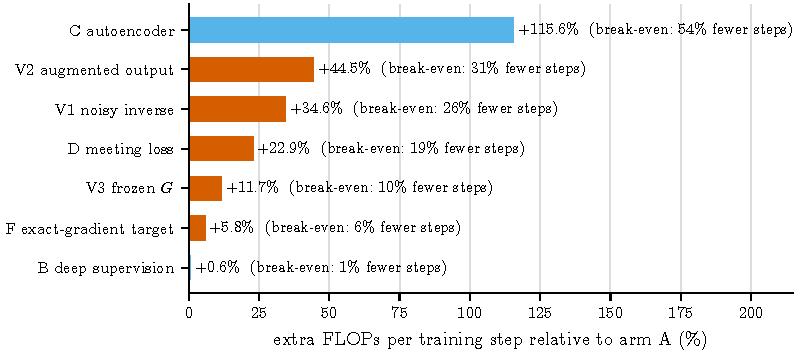
\includegraphics[width=0.78\textwidth]{fig_overhead}
\caption{Overhead of the Study 1 arms and the fraction of steps they must save to break even. Orange: variants of the meeting loss; blue: auxiliary-loss controls.}
\label{fig:overhead}
\end{figure}
